\documentclass[a4paper,12pt]{article} % добавить leqno в [] для нумерации слева
\usepackage[a4paper,top=1.3cm,bottom=2cm,left=1.5cm,right=1.5cm,marginparwidth=0.75cm]{geometry}
%%% Работа с русским языком
\usepackage{cmap}					% поиск в PDF
\usepackage{mathtext} 				% русские буквы в фомулах
\usepackage[T2A]{fontenc}			% кодировка
\usepackage[utf8]{inputenc}			% кодировка исходного текста
\usepackage[english,russian]{babel}	% локализация и переносы

\usepackage{graphicx}

\usepackage{wrapfig}
\usepackage{tabularx}

\usepackage{hyperref}
\usepackage[rgb]{xcolor}
\hypersetup{
colorlinks=true,urlcolor=blue
}
\usepackage{multirow}
\usepackage{hhline}


%%% Дополнительная работа с математикой
\usepackage{amsmath,amsfonts,amssymb,amsthm,mathtools} % AMS
\usepackage{icomma} % "Умная" запятая: $0,2$ --- число, $0, 2$ --- перечисление

%% Номера формул
\mathtoolsset{showonlyrefs=true} % Показывать номера только у тех формул, на которые есть \eqref{} в тексте.

%% Шрифты
\usepackage{euscript}	 % Шрифт Евклид
\usepackage{mathrsfs} % Красивый матшрифт

%% Свои команды
\DeclareMathOperator{\sgn}{\mathop{sgn}}

%% Перенос знаков в формулах (по Львовскому)
\newcommand*{\hm}[1]{#1\nobreak\discretionary{}
{\hbox{$\mathsurround=0pt #1$}}{}}

\begin{document}
	
	\begin{titlepage}
	\begin{center}
		{\large МОСКОВСКИЙ ФИЗИКО-ТЕХНИЧЕСКИЙ ИНСТИТУТ (НАЦИОНАЛЬНЫЙ ИССЛЕДОВАТЕЛЬСКИЙ УНИВЕРСИТЕТ)}
	\end{center}
	\begin{center}
		{\large Физтех-школа электроники, фотоники и молекулярной физики}
	\end{center}
	
	
	\vspace{4.5cm}
	{\huge
		\begin{center}
			{Лабораторная работа 6.6.1}\\
			Исследование резонансного поглощения $\gamma$-квантов (эффект Мессбауэра)
		\end{center}
	}
	\vspace{2cm}
	\begin{flushright}
		{\LARGE Салтыкова Дарья \\
			\vspace{0.5cm}
			Б04-105}
	\end{flushright}
	\vspace{8cm}
	\begin{center}
		Долгопрудный 2024
	\end{center}
\end{titlepage}

\section{Введение}

\noindent \textbf{Цель работы:} с помощью метода доплеровского сдвига мессбауэровской линии поглощения исследовать резонансное поглощение $\gamma$-лучей, испускаемых ядрами олова $^{119}$Sn в соединении BaSnO$_3$ при комнатной температуре. Определить положение максимума резонансного поглощения, его величину, а также экспериментальную ширину линии Г$_\text{экс}$. Оценить время жизни возбужденного состояния ядра $^{119}$Sn.

\medskip
	 

\section{Теоретические сведения}
\noindent При испускании или поглощении $\gamma$-кванта ядром, находящимся в узле кристаллической решётки, могут происходить два процесса:


\noindent 1. Изменение колебательного состояния решётки, т.е. возбуждение фононов.


\noindent 2. Передача импульса $\gamma$-кванта решётке как целому, без изменения её колебательного состояния, т.е. упругое испускание и поглощение $\gamma$-кванта.


\noindent С понижением температуры вероятность упругих процессов возрастает.


\noindent Эффект Мессбауэра - явление излучения и поглощения $\gamma$-квантов в твёрдых телах без рождения фононов. Мессбауэровский переход осуществляется в том случае, если колебательное состояние решётки не изменяется и $\gamma$-квант получает всю энергию перехода.


\noindent Проведём оценки для свободного ядра. Ядро, испускающее $\gamma$-квант, приобретает импульс отдачи, равный по абсолютной величине импульсу $\gamma$-кванта. Если ядро свободно и изначально покоится, энергия отдачи $R$ равна

$$
R=\frac{p^2}{2M_n} = \frac{E_{\gamma}^2}{2M_nc^2}.
$$

\noindent В качестве примера рассмотрим ядро олова Sn-119, его расстояние между основным и первьм возбуждённьм уровнями составляет $E_{0}=23.8$ кэВ, тогда согласно закону сохранения энергии $E_{0}=E_{\gamma}+R$ и принимая $R \ll E_{\gamma}$, получаем

$$
R=\frac{E_{\gamma}^{2}}{2 M_{n} c^{2}} \approx \frac{E_{0}^{2}}{2 M_{n} c^{2}}=2.5 \cdot 10^{-3} \mathrm{ eV.}
$$

\noindent Возбуждённые уровни ядра имеют конечную ширину. Отложим по оси абсцисс энергию ядра, по оси ординат -- вероятность найти ядро с данной энергией. Ширина кривой, измеренная на половине вьсоты, назьвается естественной шириной линии Г. Она связана со средним временем жизни возбуждённого состояния ядра соотношением
неопределённостей:

$$
\Gamma \tau \approx \hbar.
$$

\noindent Ширина линий испускания и поглощения складывается из собственной ширины линии и доплеровской ширины, которая играет основную роль и связана с тепловым движением атомов. Доплеровский сдвиг уровней в нерелятивистском случае будет рассчитываться по формуле

$$
D = \frac{v}{c} E_{\gamma} \approx \frac{v}{c} E_0.
$$

\noindent На одну степень свободы ядра (движение к поглотителю или от него) приходится энергия, равная $k_\text{Б}T/2$. Приравнивая это значение к кинетической энергии ядра $M_nv^2/2$, получаем значение скорости

$$
v = \sqrt{\frac{k_{\text{Б}}T}{M_n}}.
$$

\noindent Принимая во внимание энергию отдачи, значение доплеровской ширины линии испускания Sn-119 при комнатной температуре равно

$$
D = \sqrt{2Rk_{\text{Б}}T} = 1.5 \cdot 10^{-2} \text{ eV}.
$$

\begin{figure}[h!]
\begin{center}
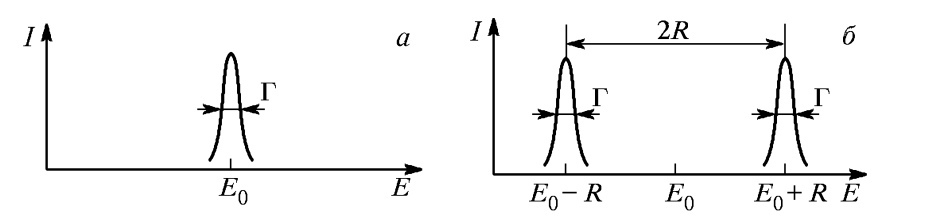
\includegraphics[scale=0.55]{1}
\caption{Энергетическое распределение, характеризующее возбужденное состояние ядра (а), и сдвиг линий испускания и поглощения из-за отдачи при свободных ядрах (б)}
\end{center}
\end{figure}


\section{Экспериментальная установка}
\noindent В ходе измерения источник остаётся неподвижен, а образец поглотителя совершает равномерное движение с контролируемой скоростью. Доплеровский сдвиг изменяет частоту гамма-квантов в системе покоя поглотителя, что позволяет изучить зависимость поглощения в образце от энергии гамма-кванта. Детектируется интенсивность $\gamma$-излучения, прошедшего через образец поглотителя. При совпадении энергии гамма-кванта с разницей энергий между основным состоянием и первым возбуждённым происходит резонансное поглощения гамма-квантов и интенсивность прошедшего излучения уменьшается. Измерительная аппаратура (сцинцилятор с ФЭУ) оптимизированы под детектирование квантов с энергией 23.8 кэВ, электронная часть схемы измерения оптимизируется под обнаружение этих квантов в ходе работы. Принципиальная схема установки представлена на рис. 2.

\begin{figure}[h!]
\begin{center}
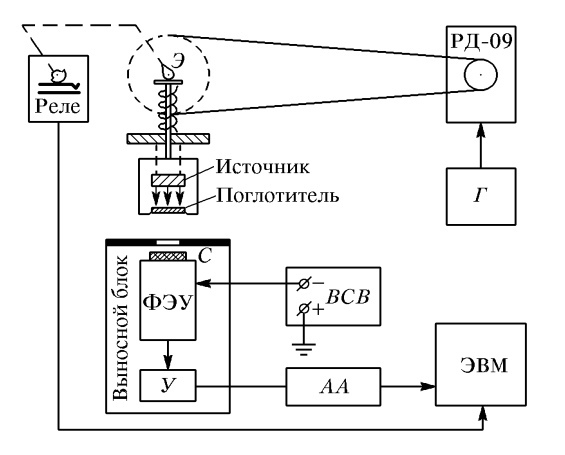
\includegraphics[scale=0.5]{2} %width = 0.7\textwidth
\caption{Блок-схема установки для наблюдения эффекта Мессбауэра: Э -- эксцентрик, С -- сцинтилляционный кристалл $\mathrm{NaI}(\mathrm{Tl})$, У -- усилитель, $\mathrm{AA}$ -- одноканальный амплитудный анализатор, ЭВМ -- персональный компьютер, Г -- генератор для питания двигателя, РД-09 -- двигатель с редуктором, ВСВ -- высоковольтный стабилизированный выпрямитель}
\end{center}
\end{figure}	

\section{Ход работы}
\subsection{Измерение спектра источника}

\textit{Цель этого этапа работы — подобрать настройки анализатора импульсов так, чтобы детектировались только гамма-кванты с энергией 23.8 кэВ, исходящие от источника $^{119}Sn$.}\\

\noindent Проведем измерения при значениях нижнего порога напряжения от 0 до 9,5В (Табл. 1, рис. 3).

\begin{flushleft}
\begin{table}[h!]
\begin{tabular}{|l|l|l|l|l|l|l|l|l|l|l|}
\hline
Промежуток измерения, В & 0     & 0,5   & 1     & 1,5   & 2     & 2,5   & 3     & 3,5   & 4     & 4,5   \\ \hline
Интенсивность, счет     & 0     & 74,8  & 17,6  & 25,6  & 76,8  & 135,6 & 178,8 & 212,8 & 244,2 & 313,2 \\ \hline
Промежуток измерения, В & 5     & 5,5   & 6     & 6,5   & 7     & 7,5   & 8     & 8,5   & 9     & 9,5   \\ \hline
Интенсивность, счет     & 392,4 & 424,2 & 371,2 & 283,6 & 186,2 & 81,6  & 34,2  & 15,8  & 8     & 3,6   \\ \hline
\end{tabular}
\label{tab}
\caption{Измерение спектра источника излучения}
\end{table}
\end{flushleft}

\begin{figure}[h!]
\begin{center}
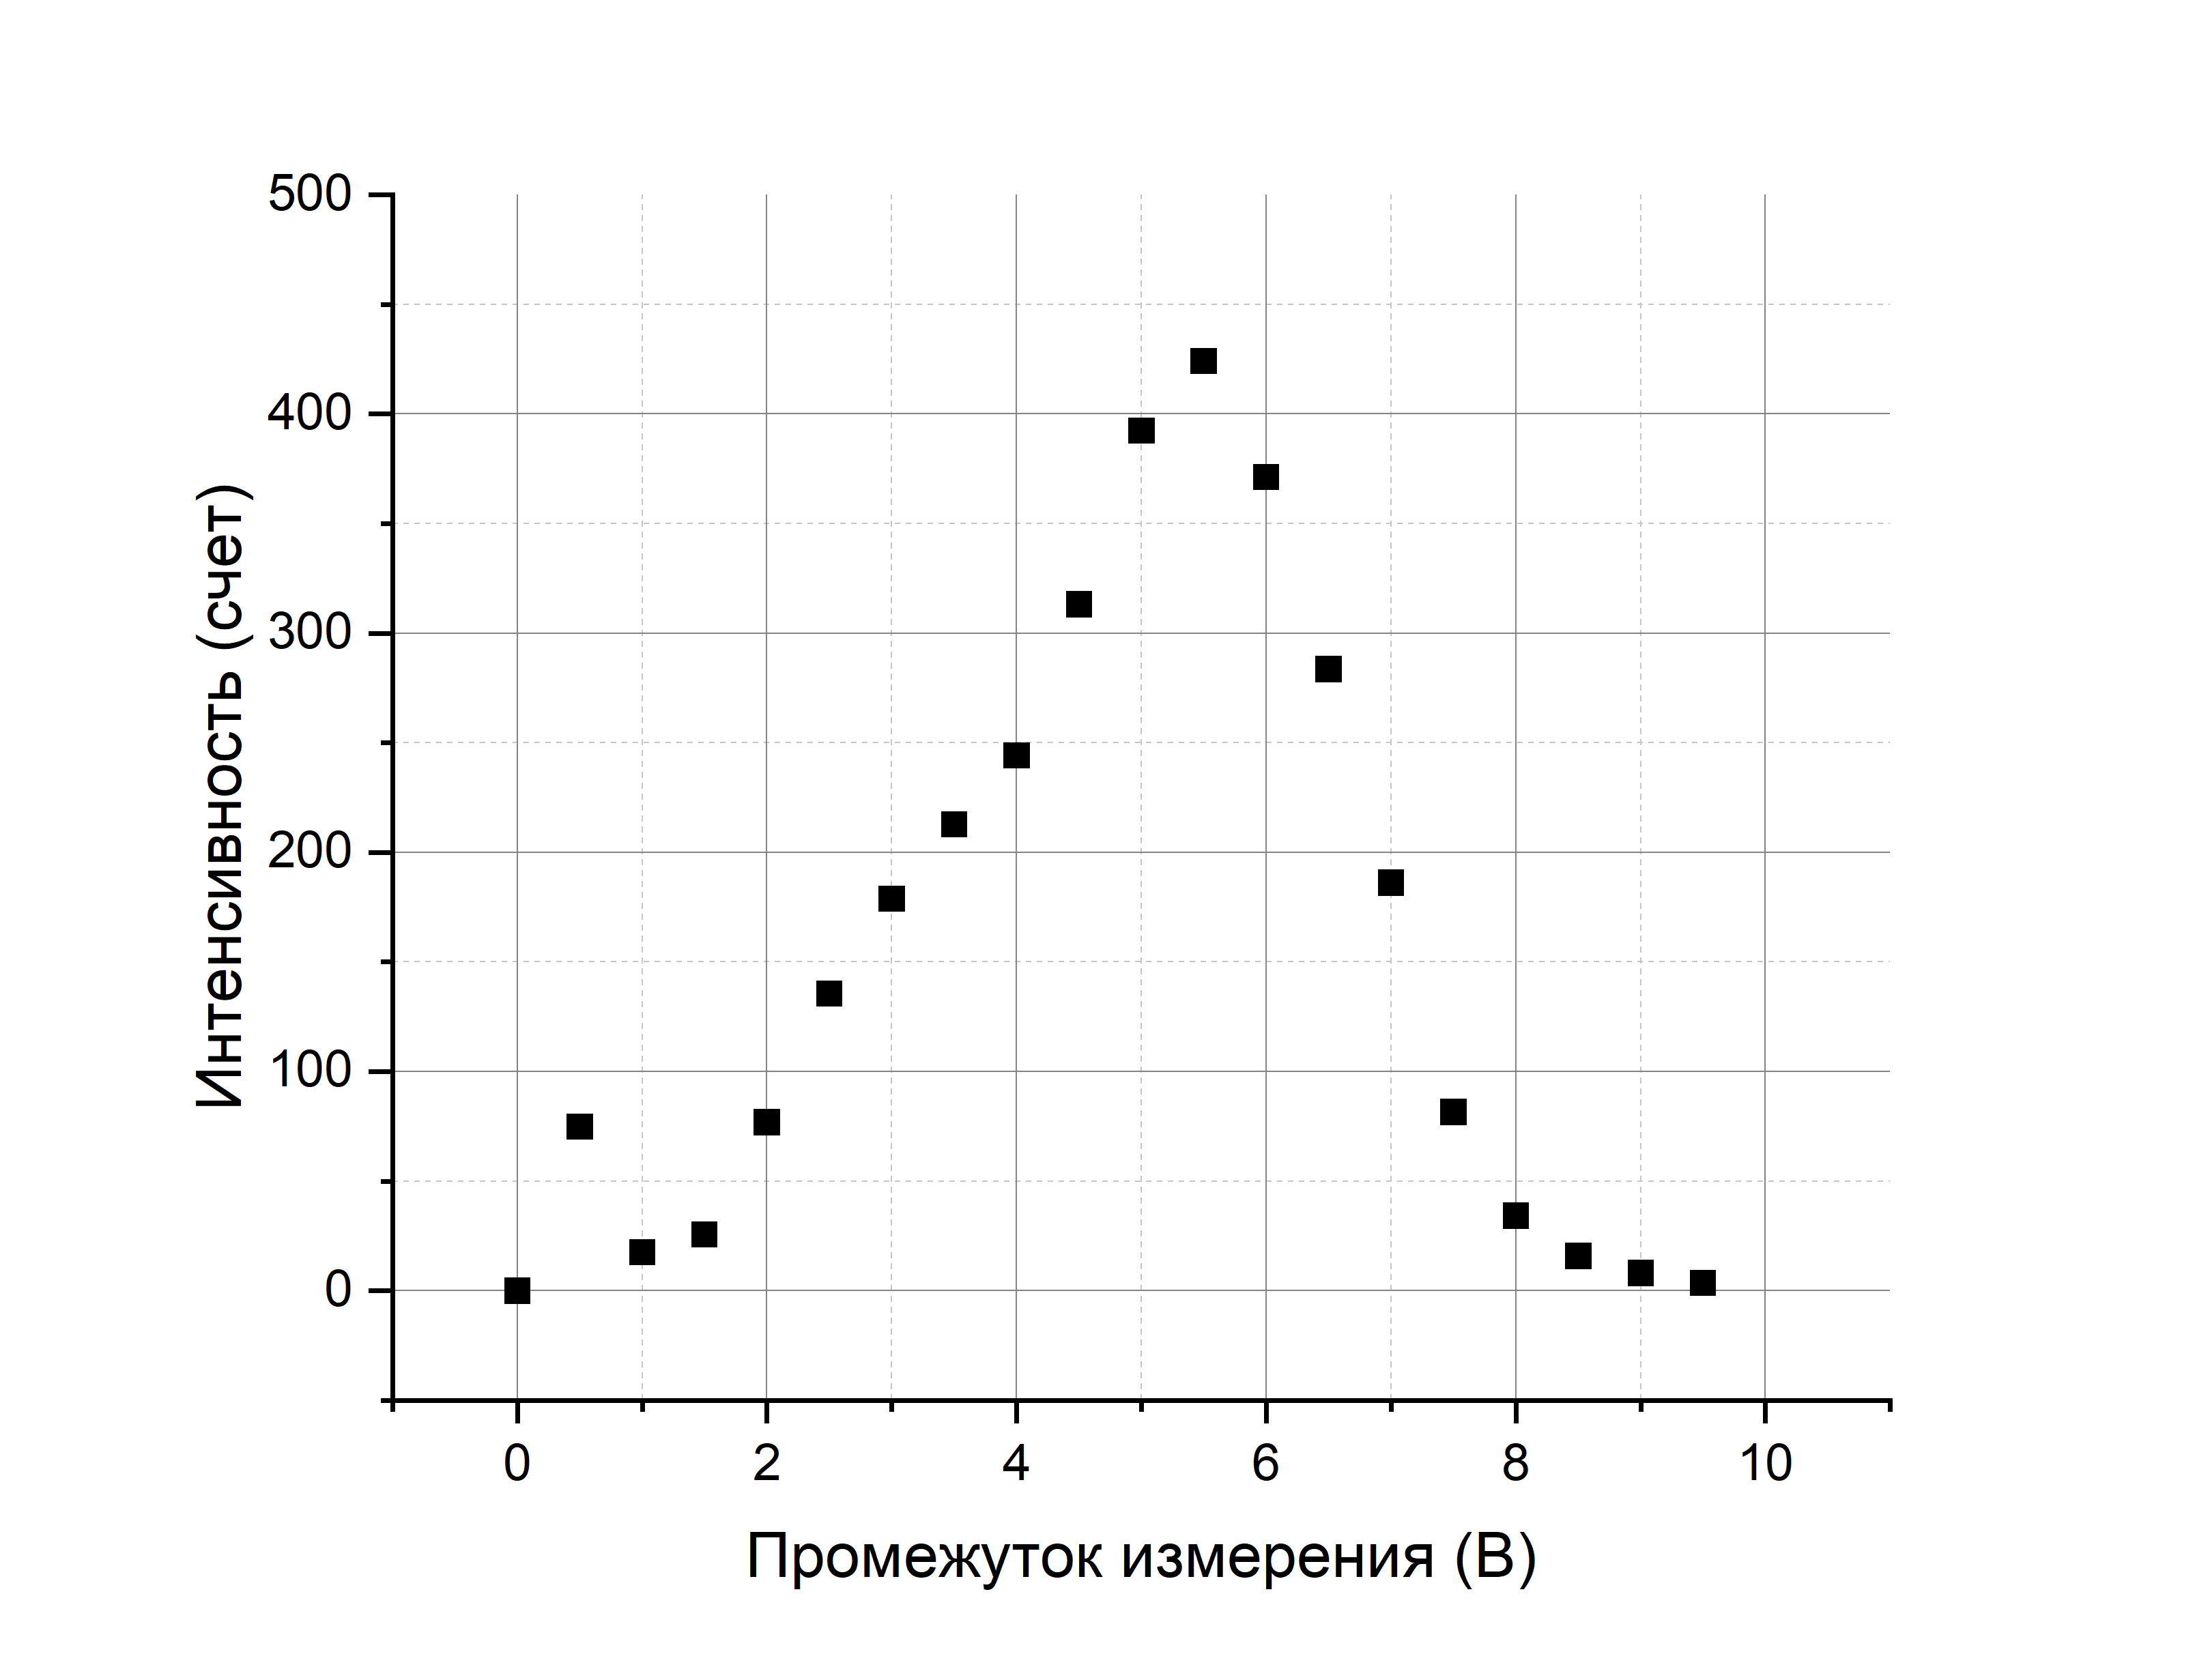
\includegraphics[scale=0.6]{spectrum.png}
\label{spectrum}
\caption{Спектр источника излучения}

\end{center}
\end{figure}

\noindent Измеренный спектр имеет колоколообразный максимум на правых 2/3 спектра - от 5 до 6В, и с фоновым сигналом на низких напряжениях. Колоколообразный максимум представляет собой аппаратно уширенную линию гамма-квантов с энергией 23.8 кэВ.\\

\noindent \textit{По окончании этого этапа электронная схема нашей установки настроена так, что подсчитываются только гамма-кванты с энергиями, соответствующими используемому источнику.}

\subsection{Измерение резонансного поглощения}

\textit{Измерим резонансное поглощение для четырёх образцов. Исследуем образцы в следующей последовательности: образец №1 (металлическое олово минимальной толщины) - толщина 90 мкм, затем образцы №2 - толщина 180 мкм, и №3 - толщина 310 мкм (металлическое олово другой толщины), образец №4 ($SnO_2$).}
\\

\noindent Для измерения фона установим время
накопления 20 секунд. Полученное значение фона: 2,05 1/сек.

\noindent Проведем серию измерений при разных скоростях движения поглотителя, чтобы
получить достаточно подробную запись линии поглощения. 

\noindent Результаты измерений представлены на графиках (Рис. 4).

\begin{figure}[h!]
\begin{minipage}[h!]{0.55\linewidth}
\center{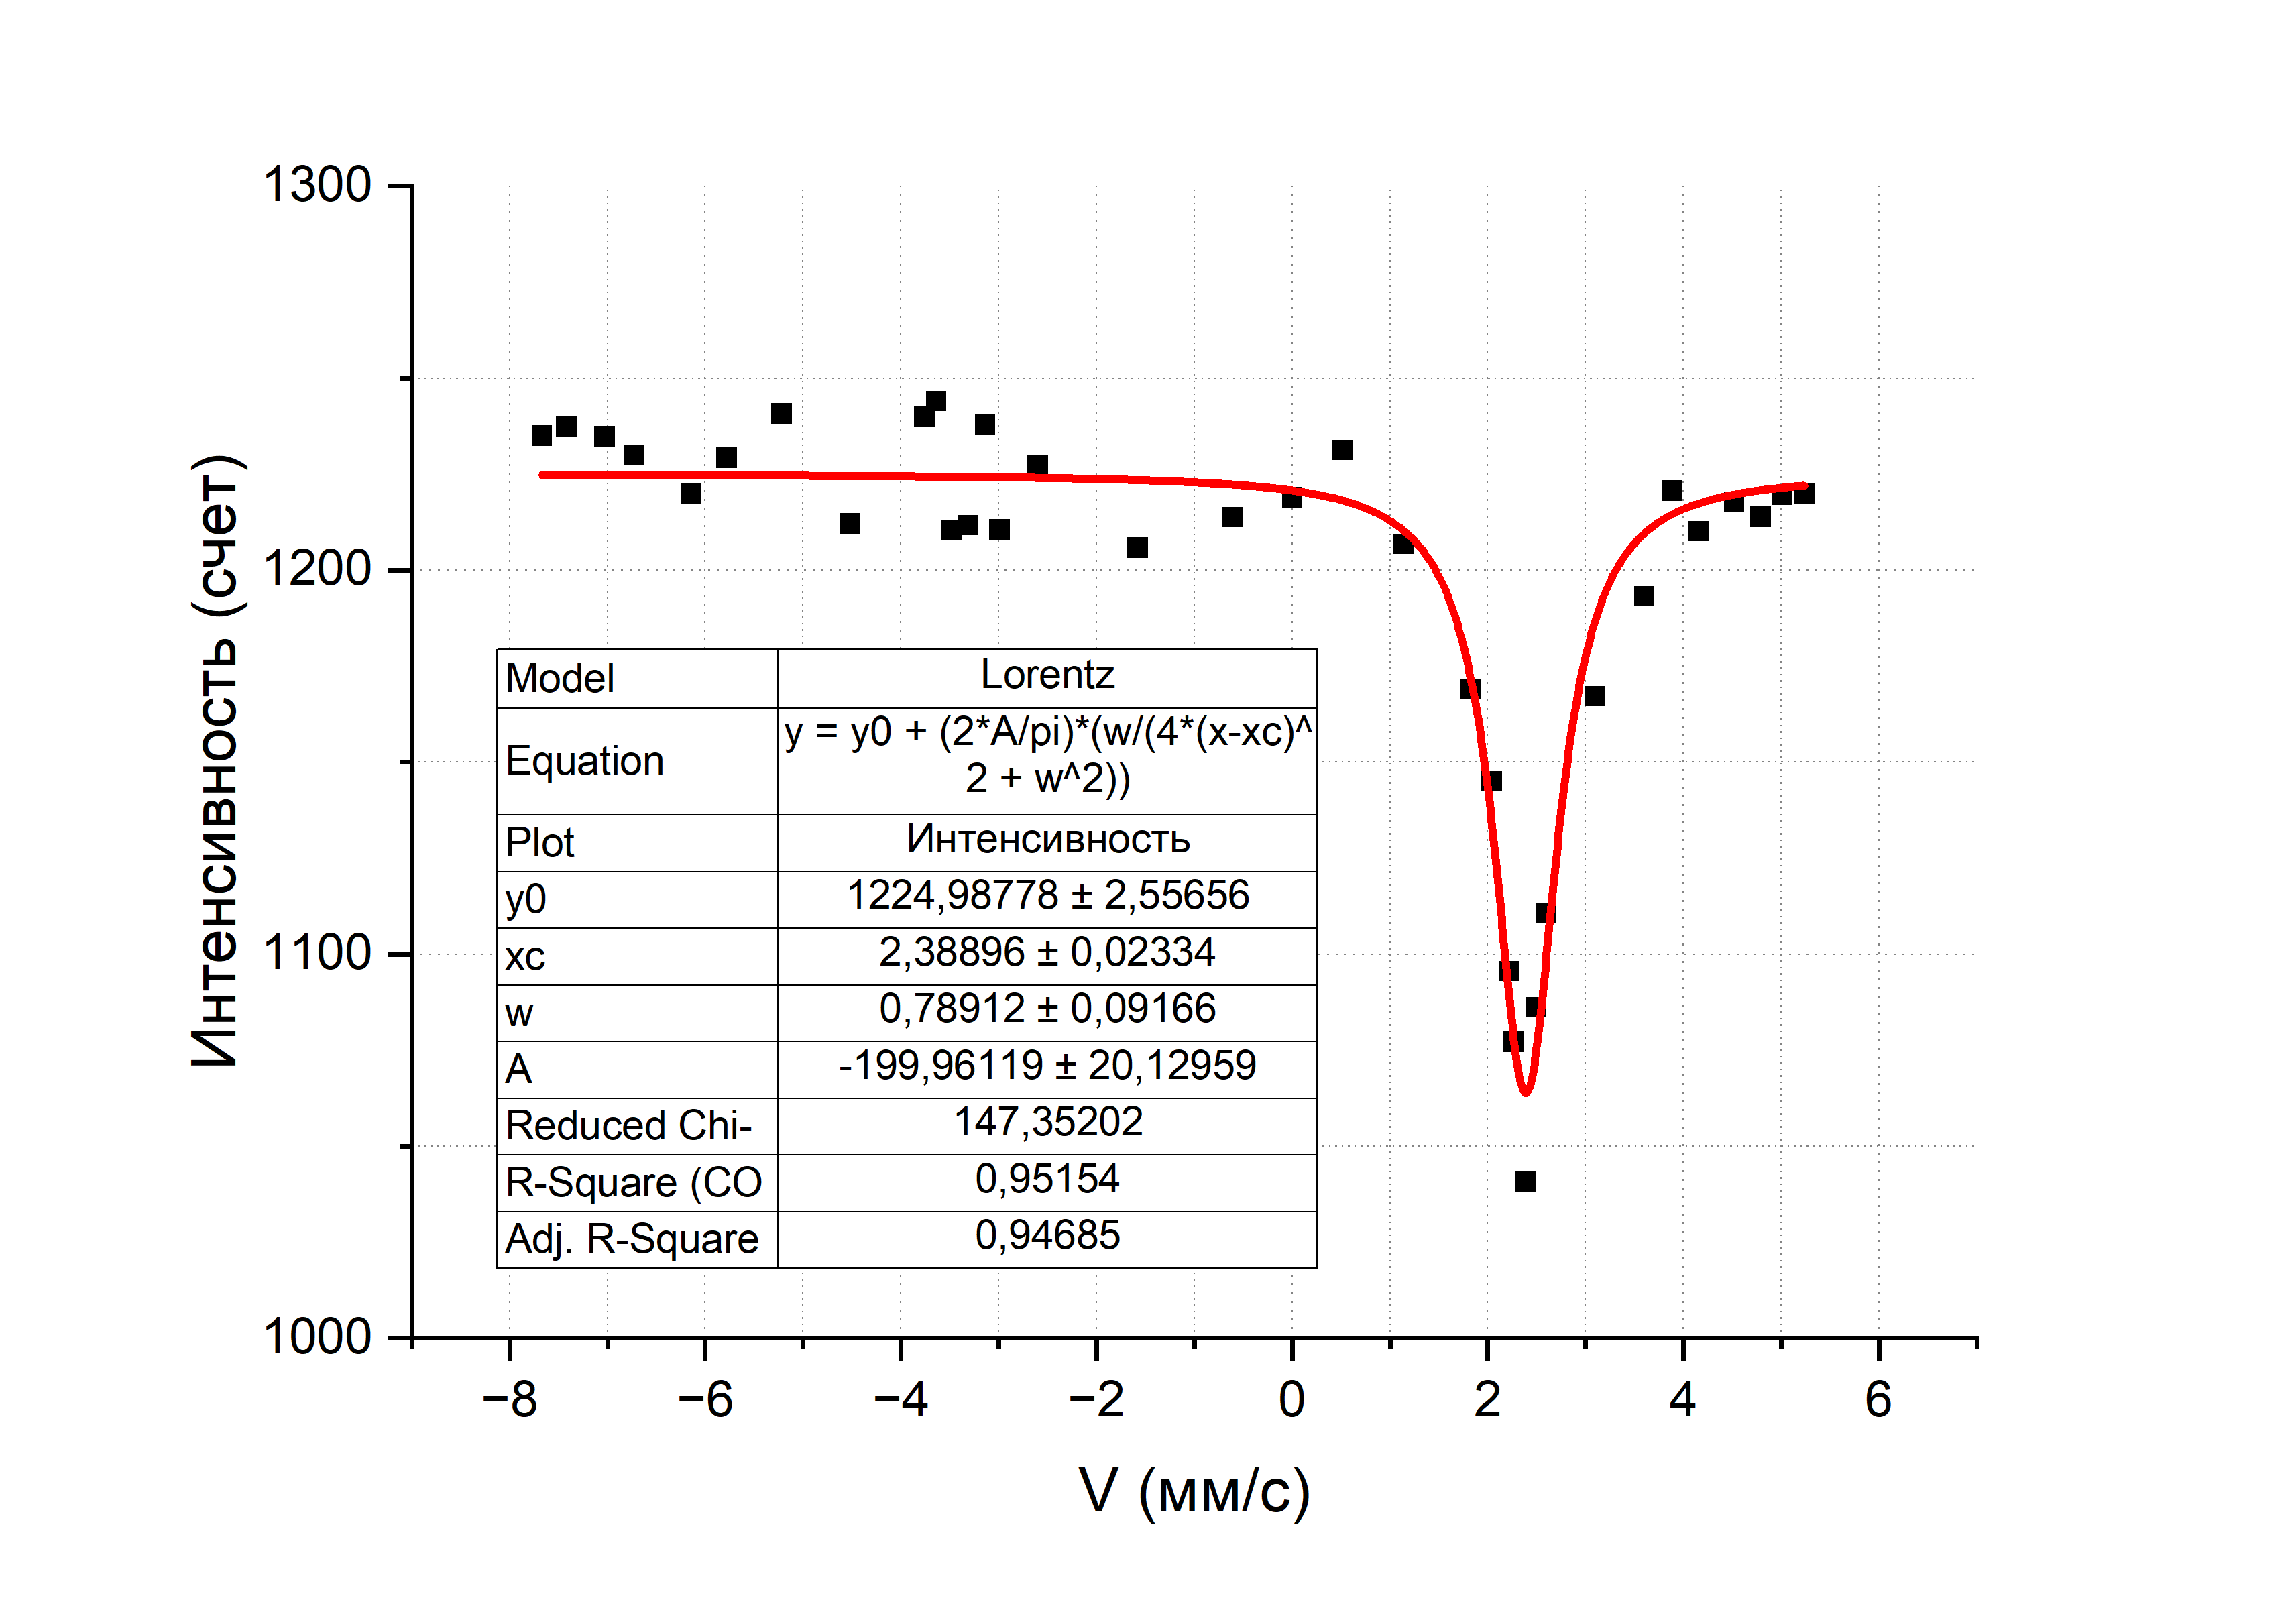
\includegraphics[width=1\linewidth]{gr1.png}} Поглотитель 1 \\
\end{minipage}
\hfill
\begin{minipage}[h!]{0.55\linewidth}
\center{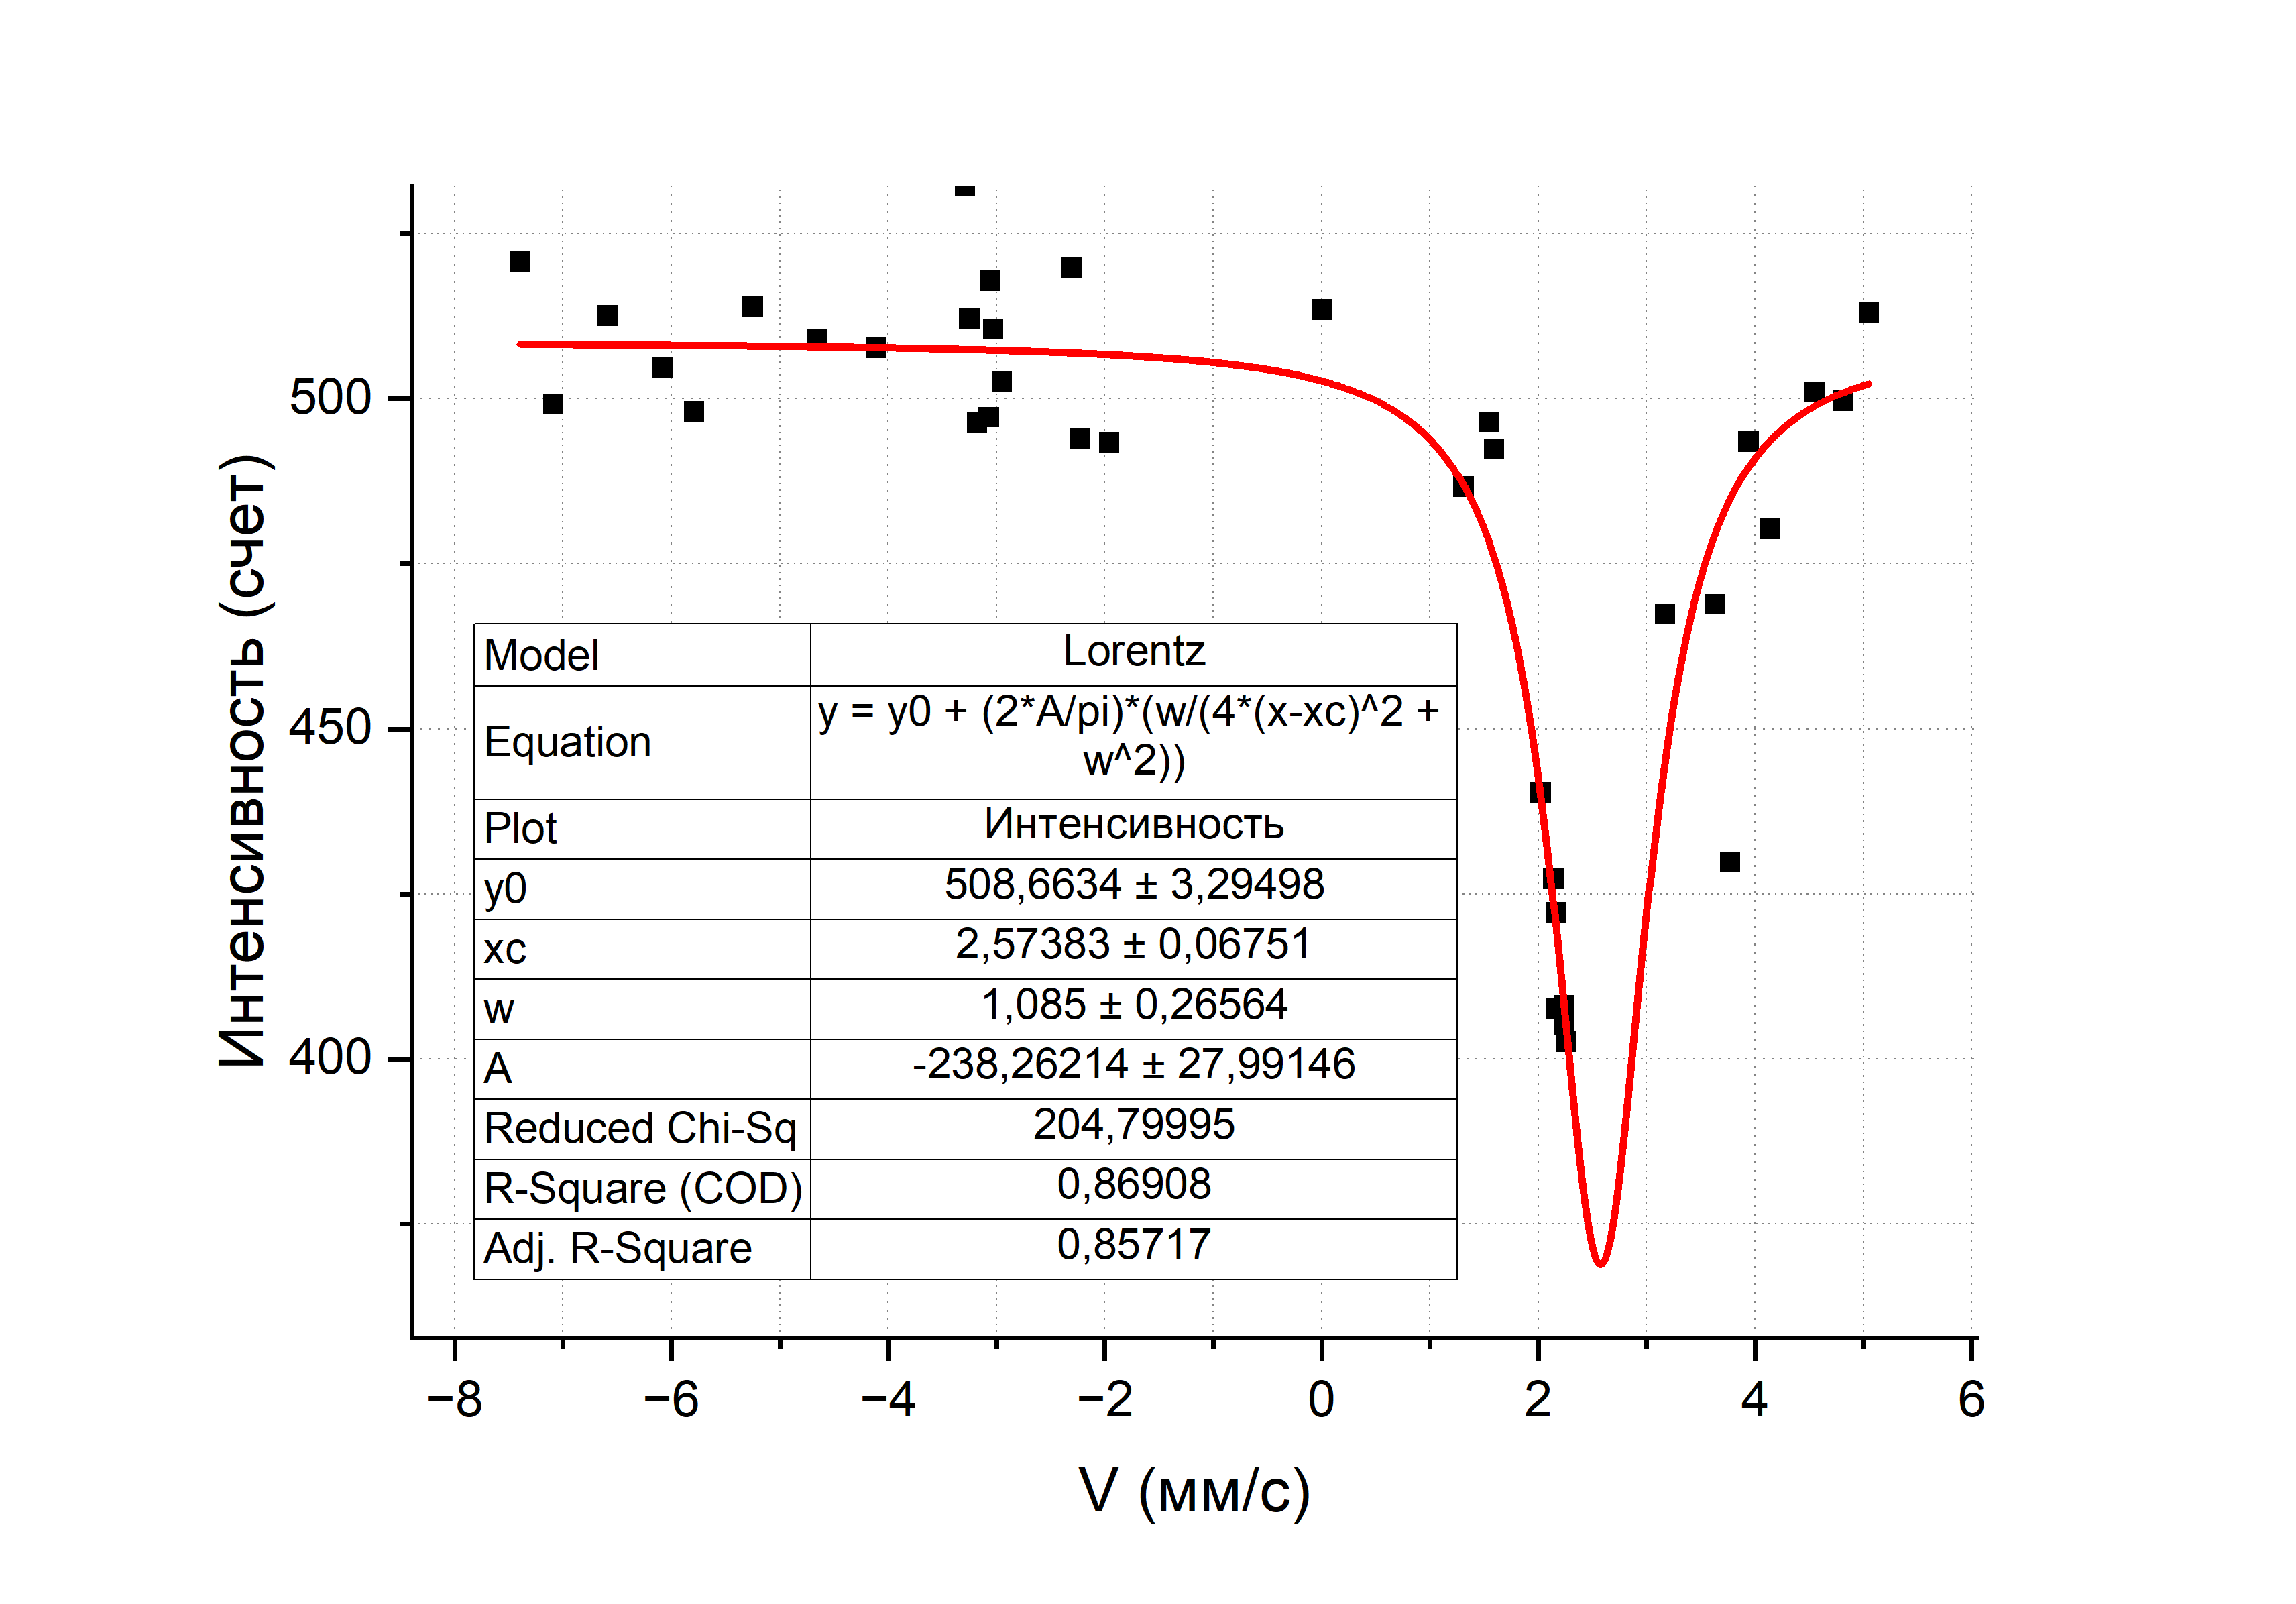
\includegraphics[width=1\linewidth]{gr2.png}} \\Поглотитель 2
\end{minipage}
\vfill
\begin{minipage}[h!]{0.55\linewidth}
\center{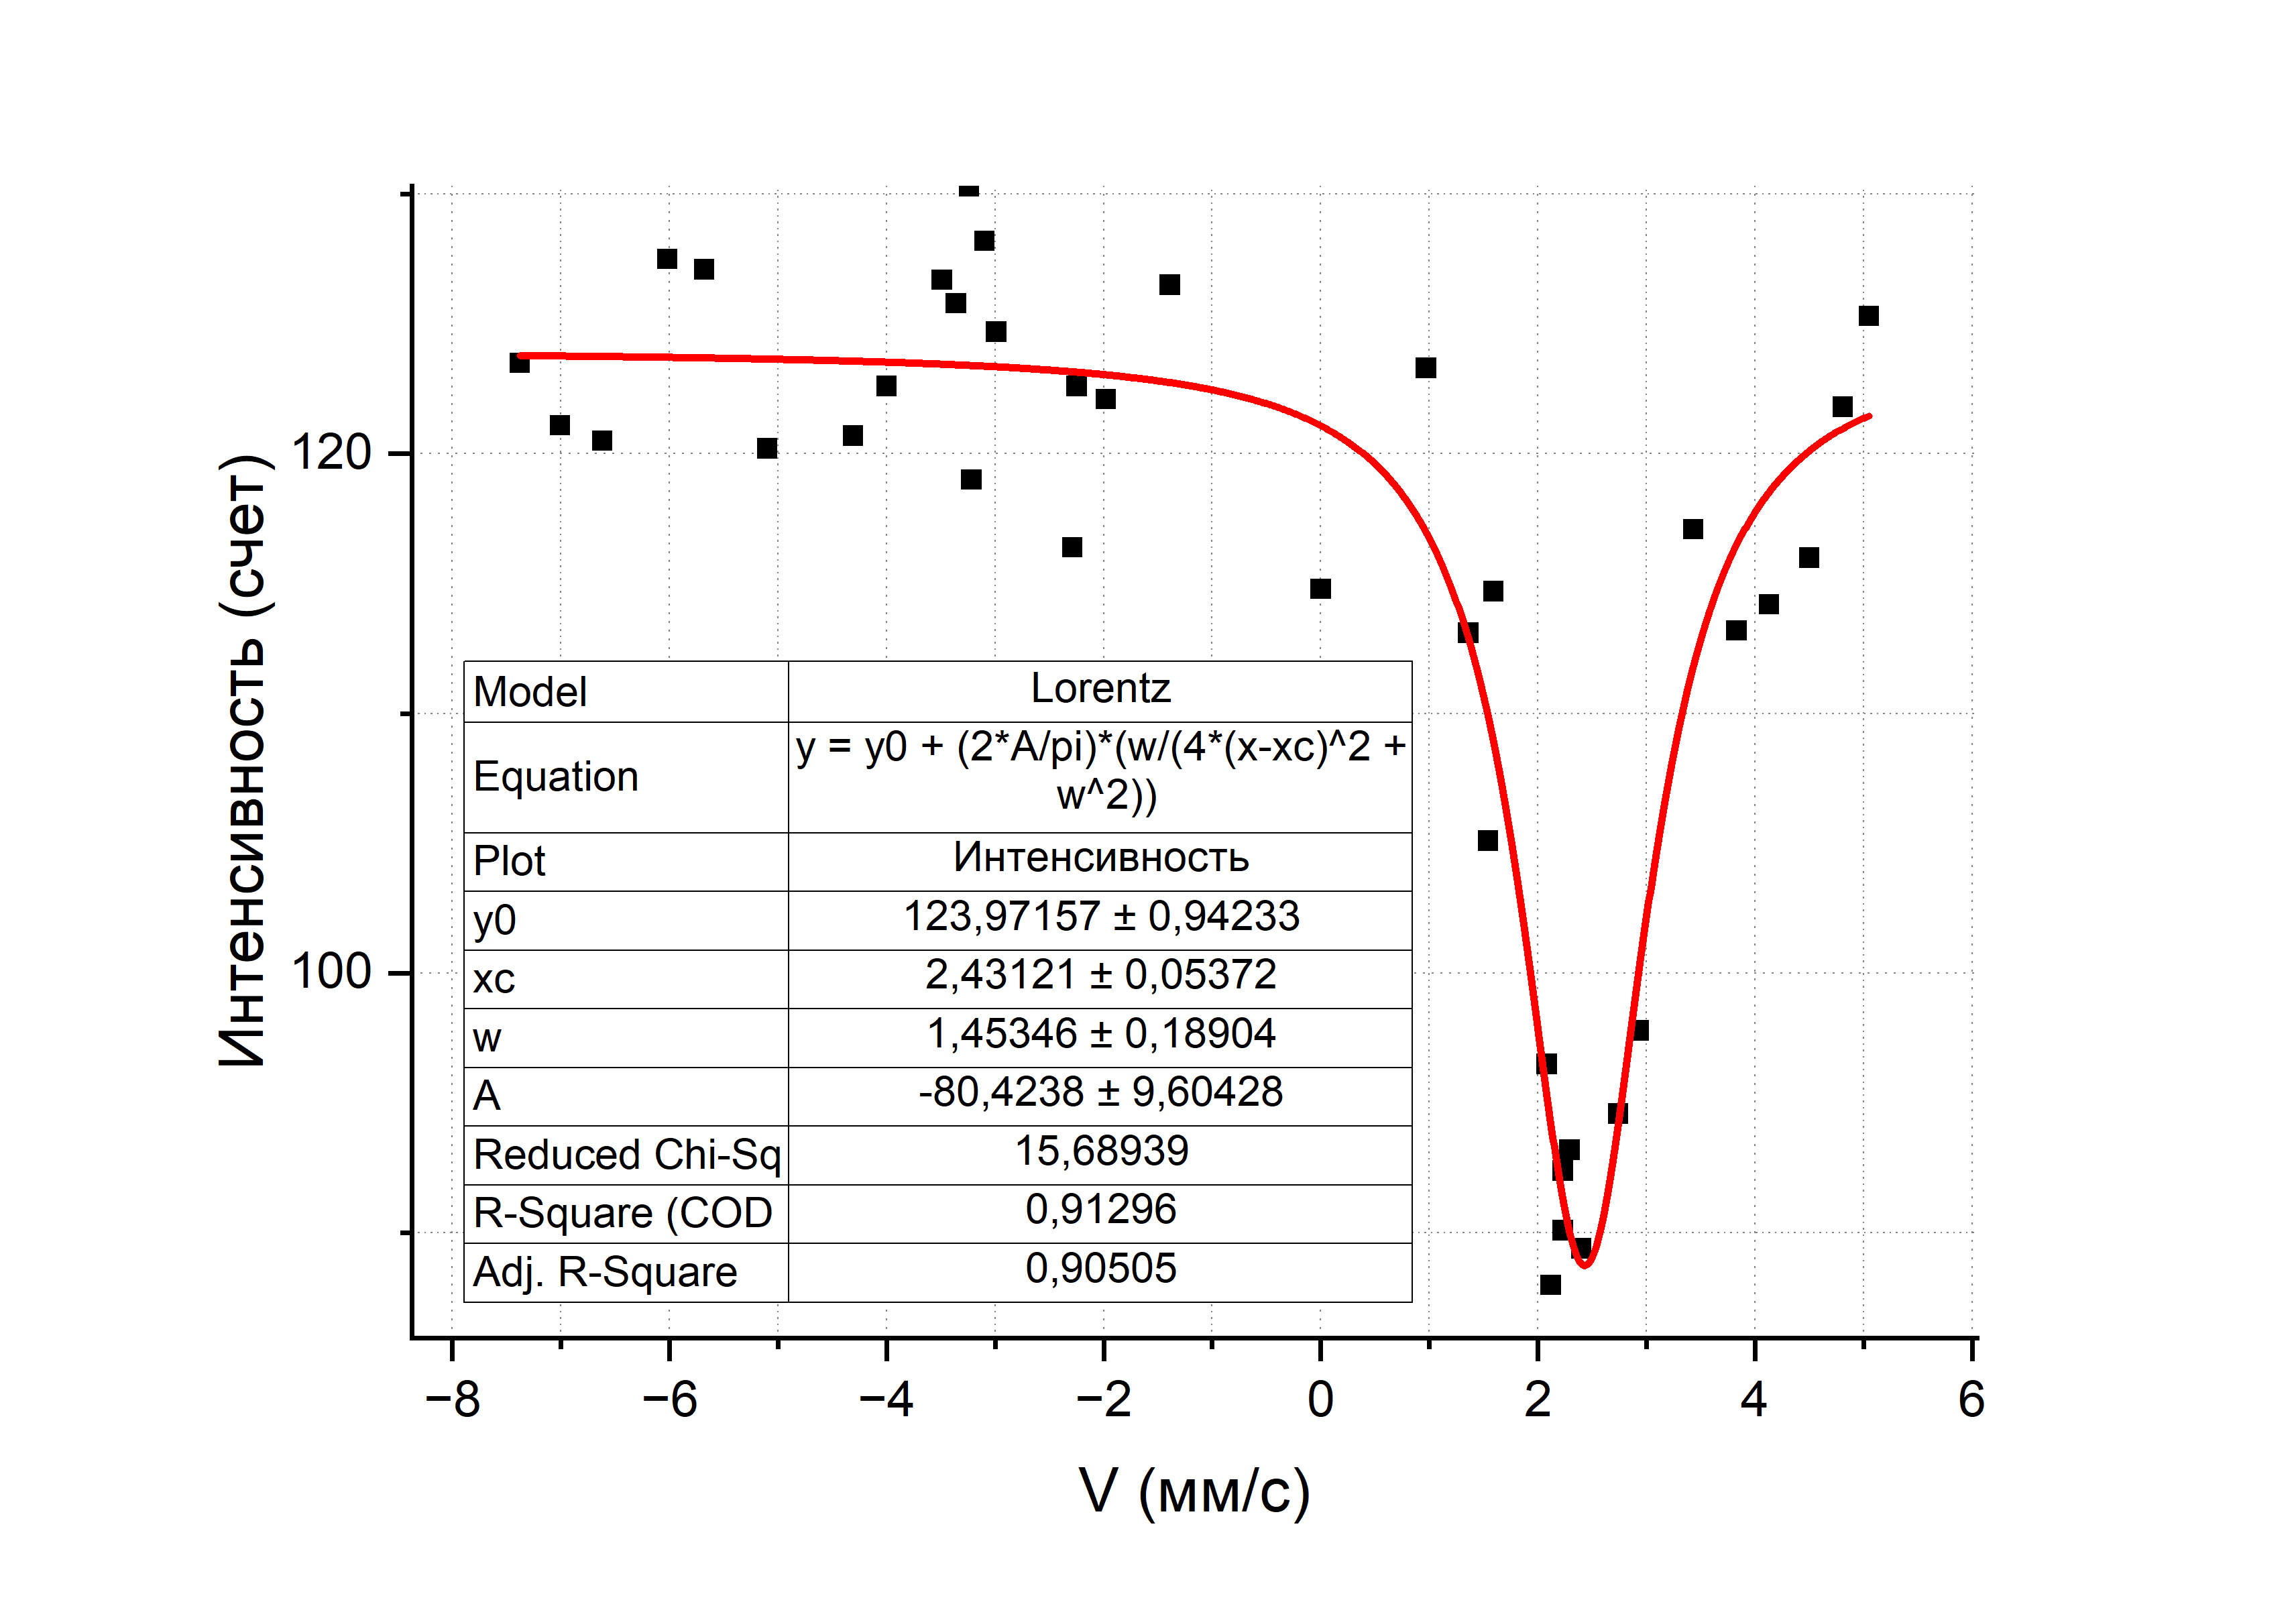
\includegraphics[width=1\linewidth]{gr3.png}} Поглотитель 3 \\
\end{minipage}
\hfill
\begin{minipage}[h!]{0.55\linewidth}
\center{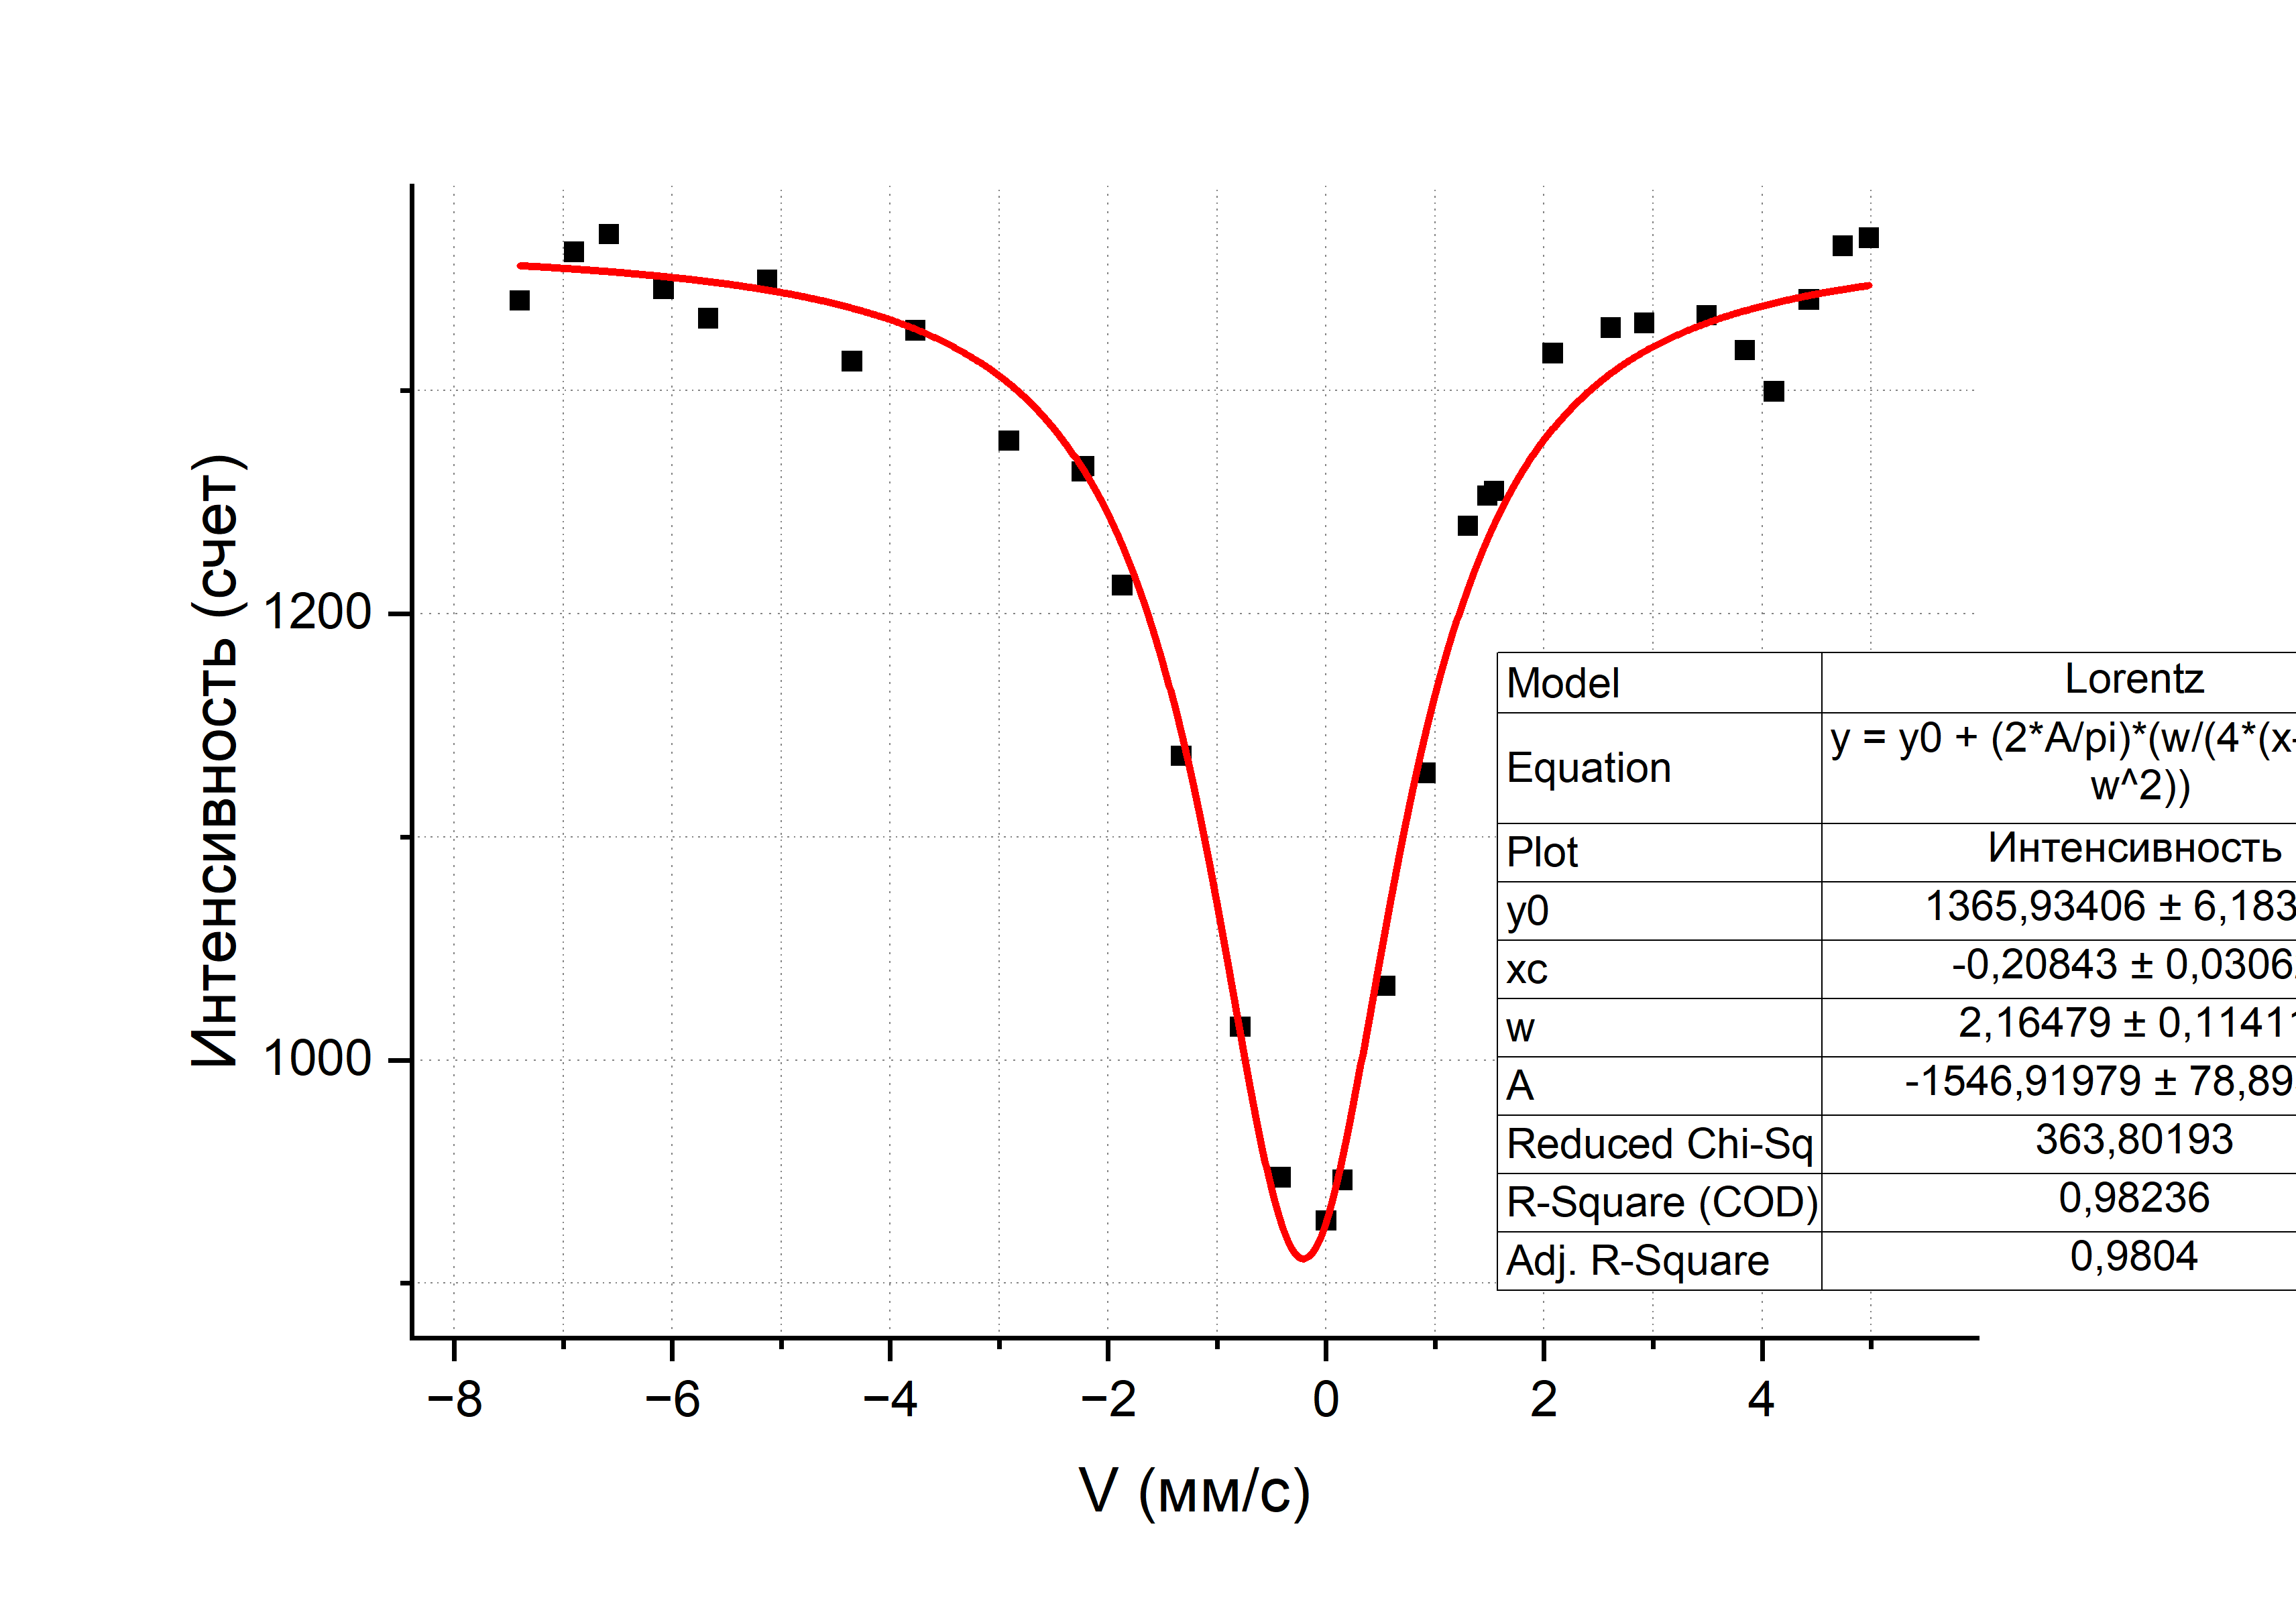
\includegraphics[width=1\linewidth]{gr4.png}} Поглотитель 4 \\
\end{minipage}
\caption{Спектры резонансного поглощения}
\label{graphs}
\end{figure}

\section{Обработка результатов}

Формула для вычисления величины амплитуды эффекта Мессбауэра:
$$
\varepsilon(v) = \frac{N(\infty) - N(v)}{N(\infty) - N_\text{ф}},
$$
\noindent где $N(\infty)$ -- скорость счёта квантов при достаточно большой скорости, $N(v)$ -- скорость счёта квантов, прошедших через поглотитель при некоторой скорости, $N_\text{ф}$ -- скорость счёта радиоактивного фона (вычитается программой автоматически).

\noindent Величина химического сдвига, выраженная в эВ:
$$
\Delta E = E \frac{v}{c},
$$
\noindent где $E$ -- энергия гамма-кванта, излучаемого веществом (в нашем случае $E$ = 23.8 кэВ).

\noindent Экспериментальная ширина линии Г$_e$, выраженная в эВ:

$$
\Gamma_e = 2 \Gamma = E \frac{v_\Gamma}{c}.
$$

\begin{table}[h!]

\begin{tabular}{|c|c|c|c|}
\hline
              & Амплитуда, \% & Хим. сдвиг, эВ       & Ширина линии, эВ     \\ \hline
Поглотитель 1 & 13,2          & $1,89 \cdot 10^{-7}$ & $6,27 \cdot 10^{-8}$ \\ \hline
Поглотитель 2 & 27,6          & $2,04 \cdot 10^{-7}$ & $8,61 \cdot 10^{-8}$ \\ \hline
Поглотитель 3 & 28,9          & $1,93 \cdot 10^{-7}$ & $1,15 \cdot 10^{-7}$ \\ \hline
Поглотитель 4 & 33,4          & $1,67 \cdot 10^{-8}$ & $1,71 \cdot 10^{-7}$ \\ \hline
\end{tabular}
\label{tab2}
\caption{Амплитуда резонансного поглощения в максимуме, величина
химического сдвига и экспериментальная ширина линии Г.}
\end{table}


\section{Вывод}

В ходе работы с помощью метода доплеровского сдвига исследовалось резонансное поглощение $\gamma$-лучей, испускаемых ядрами олова Sn-119 при комнатной температуре. Эксперимент был проведен для образцов различной толщины. В спектрах резонансного поглощения (Рис. 4) наблюдается уширение при увеличении толщины образца. Отметим также отсутствие химического сдвига у образца №4 (SnO$_2$).\\


\noindent Были найдены амплитуда резонансного поглощения в максимуме, величина
химического сдвига и ширина линии (Табл. 2). Табличное значение естественной ширины спектральной линии ядра Sn-119 составляет $3 \cdot 10^{-8}$ эВ, что совпадает по порядку величины с экспериментально полученными значениями. Различие же можно объяснить значительным влиянием доплеровского уширения при комнатной температуре.

\end{document}